\chapter{Model}
\label{cha:model}


The by us proposed user activity model with peer influence effects is described in detail in this chapter.
It is yet another extension of the activity-driven network framework by \citet{Perra2012a}, that was discussed in \cref{subsec:time-varying-network-models}.
However, it is not directly based on it, but on the work of \citet{Laurent2015}, which relies on the activity-driven framework as well.
This underlying model, which is explained in the first section of this chapter, allows for the formation of community structures and the development of strong and weak ties in the network.
These two properties are crucial conditions for the occurrence of peer influenced activity.
The additionally introduced mechanisms, which allow for peer influenced activity to actually happen in the network, are then discussed in \cref{sec:peer-influence-model} of this chapter.


%% ========================================================================
%% ========================================================================


\section{The Underlying Model}
\label{sec:underlying-model}


\subsection{Description}

Since this community-oriented model~\cite{Laurent2015} is based on the activity-driven framework by \citet{Perra2012a}, an activity potential \( a_{i} = \eta x_{i} \),  which is drawn from a suitable distribution, is assigned to each of the \( n \) nodes.
To reflect the heterogeneous activity patterns of people, a power-law distribution \( f(x) \sim x^{-\gamma} \) is selected.
The exponent for the activity potential distribution is fixed to \( \gamma = 2.7 \), which is a value that is similar to the exponent observed in real world communication networks.
The lower bound for the activity potential is set to \( \varepsilon = 10^{-3} \), and the time scaling parameter is fixed to \( \eta = 1 \), so that \( a_{i} = x_{i} \in [\varepsilon, 1] \).
Furthermore, for the sake of simplicity and without loss of generality we fix the size of the time window \( \Delta t \), and the number of generated links at each activation \( m \) to the value \( 1 \) as well.

The dynamic element of the model is basically identical to the activity-driven framework.
A node becomes active in every time window with probability equal to its activity potential and selects other nodes to interact with.
However, the intention of this model is it to produce adjustable community structures and weight-topological correlations in the integrated network.
This can ultimately be archived by changing the way the communication partners are selected once a node becomes active.
More specifically, to archive these more realistic topological properties, the following two additional social mechanisms are introduced:

\begin{enumerate}
    \item Memory effects
    \item Closure processes
\end{enumerate}


\paragraph{Memory Effects}
The first mechanism introduces memory to the nodes, in the sense that nodes remember all previous interactions with other nodes.
This idea was adapted from the work of \citet{Karsai2014}, and enables the formation of strong ties (i.e., interactions that are repeated often) and weak ties (i.e., interactions that area repeated infrequently) between the nodes.
This heterogeneity of tie strengths is an important role for processes that take place in many real world networks.
For instance, they showed in their original paper that strong ties are able to slow down the spreading of rumors in networks of social interactions (e.g., a network of phone calls).
This counter intuitive result can be explained by the observation that most activity is concentrated and contained in strongly tied groups, which inhibits a fast spreading of the rumor into other parts of the network.

The memory of a node is represented by a weighted egocentric network that includes all other nodes, which were already part of one or more interactions in the past.
These previous communication partners are also called neighbors.
The weight represents the number of previous interactions scaled by the link-reinforcement constant \( \delta \).
More specifically, the weight is set to \( 1 \) for the first contact and incremented by \( \delta \) for every additional contact.
\Cref{fig:egocentric-network} shows an exemplary egocentric network of the node \( v_{i} \) and its neighbors.


\begin{figure}
    \centering

    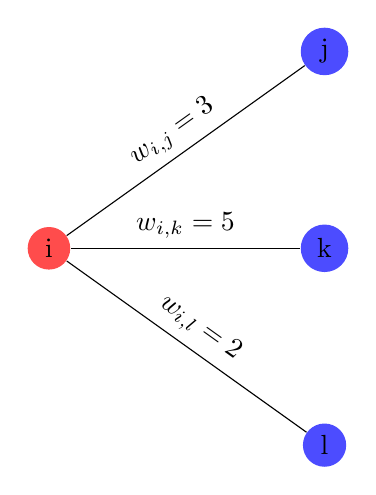
\begin{tikzpicture}[node/.style={circle,fill=red!70,minimum size=1em,inner sep=3pt]}, neighbor/.style={circle,fill=blue!70,minimum size=1em,inner sep=3pt]}]
      \node[node] (1) at (-1, -1)  {i};
      \node[neighbor] (2) at (2.5, 1.5) {j};
      \node[neighbor] (3) at (2.5, -1) {k};
      \node[neighbor] (4) at (2.5, -3.5) {l};

      \draw (1) -- (2) node [midway, above, sloped] (a) {$w_{i,j} = 3$};
      \draw (1) -- (3) node [midway, above, sloped] (b) {$w_{i,k} = 5$};
      \draw (1) -- (4) node [midway, above, sloped] (c) {$w_{i,l} = 2$};
    \end{tikzpicture}

    \caption[Egocentric network example]{Egocentric network of the node \( v_{i} \) (red node) and its neighbors \( v_{j} \), \( v_{k} \), and \( v_{l} \) (blue nodes). The link-reinforcement increment in this example is set to \( \delta = 1 \). This means that the weights exactly correspond to the number of previous interactions between the nodes.}
\label{fig:egocentric-network}
\end{figure}


The choice of a node between forming a new tie and reinforcing an existing one depends on the number of its neighbors.
This corresponds to the observations in social interaction dynamics, where actors tend to communicate almost exclusively within their social cycle, which has a limited size, due to cognitive capacities of the actors~\cite{Dunbar1992}.
Let \( k_{i} = d(v_{i}) \) be the degree of the node \( v_{i} \) in its egocentric network.
The probability for a node to form a new tie is given by \( p(k_{i}) = \sfrac{c}{(k_{i} + c)} \), and the probability to reinforce an already established tie is \( \bar{p}(k_{i}) = 1 - p(k_{i}) = \sfrac{k_{i}}{(k_{i} + c)} \), where the constant \( c \) determines the memory strength of an actor (cf.  \cref{fig:reinforcement-process-prob-plot} for details).
Therefore, the probability for the formation of a new tie decays very fast with increasing size of the egocentric network.
The memory strength constant is fixed to \( c = 1 \) in the context of our work.

If an active node decides to reinforce an existing tie, the neighbor is selected at random with respect to its tie strength.
Therefore, the probability for node \( v_{j} \) to be selected as communication partner by node \( v_{i} \) is given by
\( p_{i,j} = \sfrac{w_{i,j}}{\sum_{k \in N(v_{i})} w_{i, k}} \), where \( w_{i,j} \) denotes the tie strength between node \( v_{i} \) and \( v_{j} \) in the egocentric network of \( v_{i} \).
This reinforcement process allows for the introduction of dependencies between successive interactions of node pairs and replaces the approach from the original activity-driven framework of selecting a communication partner uniformly at random.


\myfig{reinforcement-process-prob-function}
      {width=0.75\textwidth}
      {Plots of the function that determines the probability for the formation of a new tie based on the degree of a node \( p(k) \) for different values of the memory strength \( c \). This constant can be used to model different types of users. Larger values may correspond to social explorers, that are more prone to form new ties, and smaller values are related to social keepers, which communicate almost exclusively to peers in their social circle.}
      {Probability distribution for the formation of new ties.}
      {fig:reinforcement-process-prob-plot}


\paragraph{Closure Processes}
The second mechanism introduces two different closure processes to the model.
The first one, \emph{cyclic closure}, assures the formation of triangles (i.e., cliques between three nodes), which were linked to the formation of community structures networks by \citet{Bianconi2014}.
They showed that this mechanism is sufficient to generate networks with complex topological structures (e.g., long-tailed degree distributions), in which the strength of communities depends on the cyclic closure probability.
If a node wants to form a new tie, it tries to perform a cyclic closure with probability \( p_{\Delta} \), by interacting with a randomly selected neighbor of a neighbor.

The second closure process, \emph{focal closure}, tries to emulate the social dynamic that users tend to form ties with other users that are similar to them (e.g., if they share common interests).
This process is performed whenever a new tie should be created with a probability of \( 1 - p_{\Delta} \) or if there are no suitable candidates for a cyclical closure available.
This is, for instance, the case if a node becomes active for the first time.
The weight of a new tie is always initialized to \( 1 \), regardless of the type of closure that was used to establish the new tie.

The actual implementation of these two closure mechanisms was adapted from the work of \citet{Kumpula2007}, who used the same closure mechanisms to study the formation of community structures in weighted static networks.
They model cyclic closure as a biased local search (cf. \cref{fig:cyclic-closure} for details) and focal closure as an unbiased global search, which means selecting a new node uniformly at random from the entire network.
Furthermore, they introduced a node deletion mechanism, which was adapted in this model as well.


\begin{figure}
    \centering

    \begin{subfigure}[t]{0.3\textwidth}
    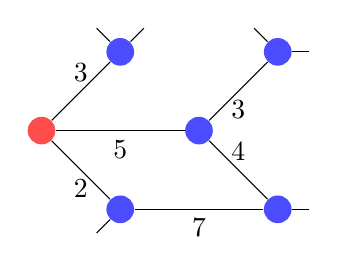
\begin{tikzpicture}[active/.style={circle,fill=red!70,minimum size=1em,inner sep=3pt]}, neighbor/.style={circle,fill=blue!70,minimum size=1em,inner sep=3pt]}]
      \node[active]   (1) at (0, 1) {};
      \node[neighbor] (2) at (1, 0) {};
      \node[neighbor] (3) at (1, 2) {};
      \node[neighbor] (4) at (2, 1) {};
      \node[neighbor] (5) at (3, 0) {};
      \node[neighbor] (6) at (3, 2) {};

      % dangling edges
      \draw (3) -- (1.3, 2.3);
      \draw (3) -- (0.7, 2.3);
      \draw (2) -- (0.7, -0.3);
      \draw (6) -- (2.7, 2.3);
      \draw (5) -- (3.4, 0);
      \draw (6) -- (3.4, 2);

      \draw (1) -- (2) node [midway, below] (a) {2};
      \draw (1) -- (3) node [midway, above] (b) {3};
      \draw (1) -- (4) node [midway, below] (c) {5};
      \draw (4) -- (6) node [midway, below] (d) {3};
      \draw (4) -- (5) node [midway, above] (e) {4};
      \draw (2) -- (5) node [midway, below] (f) {7};
    \end{tikzpicture}
    \caption{}
    \label{subfig:cyclic-closure-a}
    \end{subfigure}
    \begin{subfigure}[t]{0.3\textwidth}
    ~
    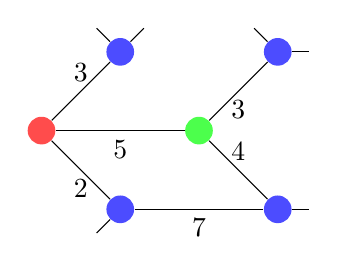
\begin{tikzpicture}[active/.style={circle,fill=red!70,minimum size=1em,inner sep=3pt]}, neighbor/.style={circle,fill=blue!70,minimum size=1em,inner sep=3pt]}, selected/.style={circle,fill=green!70,minimum size=1em,inner sep=3pt]}]
      \node[active]   (1) at (0, 1) {};
      \node[neighbor] (2) at (1, 0) {};
      \node[neighbor] (3) at (1, 2) {};
      \node[selected] (4) at (2, 1) {};
      \node[neighbor] (5) at (3, 0) {};
      \node[neighbor] (6) at (3, 2) {};

      % dangling edges
      \draw (3) -- (1.3, 2.3);
      \draw (3) -- (0.7, 2.3);
      \draw (2) -- (0.7, -0.3);
      \draw (6) -- (2.7, 2.3);
      \draw (5) -- (3.4, 0);
      \draw (6) -- (3.4, 2);

      \draw (1) -- (2) node [midway, below] (a) {2};
      \draw (1) -- (3) node [midway, above] (b) {3};
      \draw (1) -- (4) node [midway, below] (c) {5};
      \draw (4) -- (6) node [midway, below] (d) {3};
      \draw (4) -- (5) node [midway, above] (e) {4};
      \draw (2) -- (5) node [midway, below] (f) {7};
    \end{tikzpicture}
    \caption{}
    \label{subfig:cyclic-closure-b}
    \end{subfigure}
    ~
    \begin{subfigure}[t]{0.3\textwidth}
    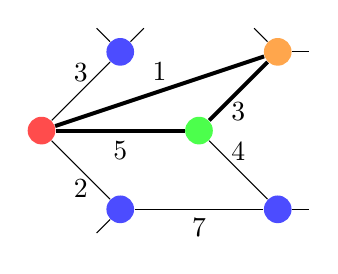
\begin{tikzpicture}[active/.style={circle,fill=red!70,minimum size=1em,inner sep=3pt]}, neighbor/.style={circle,fill=blue!70,minimum size=1em,inner sep=3pt]}, selected1/.style={circle,fill=green!70,minimum size=1em,inner sep=3pt]}, selected2/.style={circle,fill=orange!70,minimum size=1em,inner sep=3pt]}]
      \node[active]   (1) at (0, 1) {};
      \node[neighbor] (2) at (1, 0) {};
      \node[neighbor] (3) at (1, 2) {};
      \node[selected1] (4) at (2, 1) {};
      \node[neighbor] (5) at (3, 0) {};
      \node[selected2] (6) at (3, 2) {};

      % dangling edges
      \draw (3) -- (1.3, 2.3);
      \draw (3) -- (0.7, 2.3);
      \draw (2) -- (0.7, -0.3);
      \draw (6) -- (2.7, 2.3);
      \draw (5) -- (3.4, 0);
      \draw (6) -- (3.4, 2);

      \draw (1) -- (2) node [midway, below] (a) {2};
      \draw (1) -- (3) node [midway, above] (b) {3};
      \draw[line width=0.5mm] (1) -- (4) node [midway, below] (c) {5};
      \draw[line width=0.5mm] (4) -- (6) node [midway, below] (d) {3};
      \draw (4) -- (5) node [midway, above] (e) {4};
      \draw (2) -- (5) node [midway, below] (f) {7};
      \draw[line width=0.5mm] (1) -- (6) node [midway, above] (g) {1};
    \end{tikzpicture}
    \caption{}
    \label{subfig:cyclic-closure-c}
    \end{subfigure}

    \caption[Cyclic closure mechanism example]{This is an illustration of the cyclic closure mechanism of the model. The network depicted in these figures is part of the union of all egocentric networks (i.e., the integrated network). (\subref{subfig:cyclic-closure-a}) shows the active node in red. In the first step, this node has to select one of his neighbors. This is done at random with respect to the tie strengths. Therefore, the probabilities for the three neighbors to be selected are \(\sfrac{3}{10}\), \(\sfrac{5}{10}\), and \(\sfrac{2}{10}\) respectively. In this example the neighbor with the highest probability was selected, which is depicted in (\subref{subfig:cyclic-closure-b}) (green node). Since the selected neighbor has neighbors himself that do not share a link with the active node yet, the cyclic closure can be completed. This is done once more by selecting one of the candidates at random with respect to the weight of the ties and creating a new tie with unit strength with probability \( p_{\Delta} \). (\subref{subfig:cyclic-closure-c}) shows they selected node (orange node) and the newly formed triangle in the network.}
\label{fig:cyclic-closure}
\end{figure}


\paragraph{Node Deletion Mechanism}
In the activity-driven framework, nodes live forever and are, therefore, forever part of the network.
However, in this extended version of the model, nodes have an intrinsic probability \( p_{d} \) to be removed in every time step, which is the same for every node in the network.
This ensures that the network can reach a stable state, in which the structural characteristics (e.g., the community structures) become invariant in time.
Every time a node is removed from the network, a new one joins to keep the size of the network constant.
The deletion probability of nodes determines how fast the network reaches its equilibrium.
A small value for \( p_{d} \) allows for nodes to stay a long time in the network and even nodes with relatively small activity potential can become fully integrated in the community structures.
Therefore, it takes longer to reach the time invariant state if the low activity nodes are not removed fast enough.

The expected time that a node will be part of the network can be determined by viewing a nodes' lifetime as a simple Bernoulli process.
In each iteration a biased coin is tossed for every node.
The outcome of this Bernoulli random experiment determines if the node stays in the network or is replaced in the next round.
The probability for a node to be deleted after exactly \( x \) iterations is \( \prob{x} = p_{d} {(1 - p_{d})}^{x-1} = p_{d} \bar{p}_{d}^{x-1} \).
Hence, the expected value for the lifetime of a node is given by \( \expval{x} = \sum_{x=1}^{\infty} x \prob{x} = \sum_{x=1}^{\infty} x p_{d} \bar{p}_{d}^{x-1} = p_{d} \sum_{x=1}^{\infty} x \bar{p}_{d}^{x-1} \).
This sum is related to the sum of the geometric series \( \sum_{x=0}^{\infty} r^{x} = \frac{1}{1 - r} \), for \(|r| < 1 \), by being its first derivative\footnote{The first derivative of the sum of the geometric series is \( \frac{\mathrm{d} \sum_{x=0}^{\infty} r^{x}}{\mathrm{d} r} = \sum_{x=0}^{\infty} \frac{\mathrm{d} r^{x}}{\mathrm{d} r} = \sum_{x=1}^{\infty} x r^{x-1} = \frac{\mathrm{d} \frac{1}{1-r}}{\mathrm{d} r} = \frac{1}{{(1 - r)}^{2}} \), for \(|r| < 1\).}.
Therefore, the expected value for the lifetime of a node is \( \expval{x} = \sfrac{p_{d}}{{(1 - \bar{p}_{d})}^{2}} = \sfrac{1}{p_{d}} \).
This means that, for example, nodes with a deletion probability of \( p_{d} = \num{5e-05} \) will be on average deleted after 20,000 iterations.


\subsection{Properties}

The properties of this model are examined by analyzing an extended version of the integrated network.
This is very similar to the basic framework, in which the temporal network is represented as a sequence of graphs.
These graphs are denoted as instantaneous networks, and the union of these networks up to a time step \( T \) is called the integrated network.
This is also true for this extension, however, the links in the integrated network have an additional weight assigned to them, which corresponds to the tie strength in the egocentric networks of the nodes.
Another equivalent way to define the integrated network is the union of all egocentric networks up to some time step \( T \).

These newly introduced mechanisms have interesting effects on how the structures on the integrated network evolve over time.
In the beginning, after nodes formed their first ties, they start to close triangles and reinforce the ties in their egocentric network.
This means that strong community structures are formed early in the process.
However, after a while more and more weak ties are introduced and fewer triangles are closed, so that the strength of the communities declines and the network reaches its equilibrium state.
As mentioned earlier, the node deletion probability can be used to control the time until the network converges, but it can also be used to tune the strength of the communities and the average degree of the network.
A smaller value for \( p_{d} \) decreased the average local clustering coefficient and increases the average degree.

The cyclic closure probability \( p_{\Delta} \) and the reinforcement increment \( \delta \) control the formation of communities as well (see \cref{fig:community-structures-in-model}).
Furthermore, like the node deletion probability, the two parameter have an effect on the average degree of the converged network.
Higher values for the cyclic closure probability or the tie reinforcement increment result in a smaller average degree.
However, the two parameter do not influence the actual (heterogeneous) distribution of the degrees in a significant way.
The tie strengths, which are power-law distributed, are not effected by \( p_{\Delta} \), and larger values for \( \delta \) only influence the length of the tail of the distribution.

Another characteristic of this model is the larger impact of the cyclic closure probability on the emerging community structures compared to the tie reinforcement increment.
This is true since \( p_{\Delta} \) effects the number of triangles directly, whereas \( \delta \) is responsible for the creation of strong ties, which increases the bias in the local search, and only assists in the process of finding suitable nodes for the triangle formation.
Additionally, the model is able to produce higher-order correlations, that are observable in real-world networks as well.
For example, weight-topology correlations (i.e., stronger ties within groups) are measurable and are dependent on \( p_{\Delta} \) and \( \delta \) as well.


\myfig{community-structures-model}
      {width=0.90\textwidth}
      {Depiction of the influence of \( p_{\Delta} \) and \( \delta \) on the resulting community structures (image borrowed from~\cite{Laurent2015}). The networks in the first row (a--c) were generated with a fixed value for the link reinforcement increment \(\delta = 1\) and varying values for the cyclic closure probability (from left to right: \( p_{\Delta} = 0.5 \), \( p_{\Delta} = 0.9 \), and \( p_{\Delta} = 0.995 \)). This shows that \( p_{\Delta} \) directly influences the strength of the communities. Furthermore, tie strength heterogeneities are observable, with strong ties within communities (darker link color) and weak ties between them (brighter link color).The second row shows networks with a fixed cyclic closure probability \( p_{\Delta} = 0.995 \) and different reinforcement constants (from left to right: \(\delta = 0\), \(\delta = 0.5\), and \(\delta = 1.5\)). This shows that a high probability for the formation of triangles is not sufficient for the formation of communities. The reinforcement process, which helps to develop strong ties, is required as well and also effects the size of the communities.}
      {Influence of \( p_{\Delta} \) and \( \delta \) on the community structures}
      {fig:community-structures-in-model}


%% ========================================================================
%% ========================================================================


\section{Peer Influence Extension}
\label{sec:peer-influence-model}


\subsection{Idea}

So far was the activity in temporal networks entirely determined by the activity-potential distribution.
Each node is assigned an intrinsic probability to become active in each round, which is drawn from this distribution.
The assignment is done only once for every node when it is created and does not change afterwards.
After that, a node can become active in an iteration of the model either by himself or by being contacted by another active node.

The process of becoming active on one's own accord does not dependent on whether or not the node was active in previous time steps.
This corresponds to a memory-less Poisson process and leads necessarily to exponentially distributed times between two consecutive activations of a node (i.e., inter-event times).
The significance of complex long-tailed inter-event time distributions in human behavior was already discussed in \cref{sec:user-activity-models}.

However, it is evident that activations caused by other nodes are not necessarily independent of previous events, due to the memory effects introduced in the model.
For example, lets assume a node with very low activity potential is part of a group of high-activity nodes with already established strong ties.
The self-activation rate of the low-activity node will be quite low, with a mean value and standard deviation of the inter-event times that is equal to the inverse of its activity probability.

Nevertheless, the other nodes in the group will fairly often select the low-active node as communication partner when they become active, due the biased local search.
This can, of course, alter the inter-event time distributions of nodes with a small activity potential in a significant way, compared to the distributions that are generated by the activity-driven framework, where the activation through other nodes happens totally at random.
This, in this case implicit, influence that nodes have on the activity of their neighbors is an interesting effect and was a starting point for our thesis.
In this section, an extension of the prior discussed underlying model with memory and closure effects is presented, which tries to model the influences of peers in the local network in a more explicit way.

The ideas for our model were heavily influenced by the work of \citet{Walk2016}.
They proposed a model that includes peer-influence effects and examine its impact on the global activity in collaboration networks.
A more detailed description of their work is located in \cref{sec:peer-influence}.
The gist of the by us proposed extension to the community-oriented activity-driven model is that a node cannot only become active on its own based on its activity potential, but also by being motivated to become active by its neighbors, that were active in the previous iteration.

Another way to look at it is that active nodes are able to influence their neighbors to become active as well in the next round.
Therefore, introducing a more explicit peer influence mechanism to the model.
This also means that a node now can become active in three different ways.
First, it can become active by himself either due to its intrinsic fixed activity probability or due to the influence of the nodes in its egocentric network, or it can become active in a passive way by being contacted by another active node.


\subsection{Description}

The peer influence that a node \( v_{i} \) receives from its neighbors is denoted as \( p_{i} \).
Like the activity potential, \( p_{i} \) is a probability for an activation as well, but instead of being fixed, it may vary in each iteration based on the number of active neighbors in the last round.
Therefore, a more appropriate notation is \( p_{i}(t) \).
To adjust how much peer influence a node can receive at most, an upper bound \( q \) is defined, such that \( \forall t: \, 0 \leq p_{i}(t) \leq q \leq 1 \).
It denotes the maximal probability for an activation motivated by the neighbors of a node.

Since the peer influence probability depends on the neighbors that were active in the last round, the information of the last activations of the nodes must be stored as well.
This is done by extending the egocentric networks to save the timestamp of the last activation for each node.
The time of last activation of \( v_{i} \) is called \( t_{i} \) and is updated independently of the type of activation (i.e., due to self activation or by being contacted by another active node).

Furthermore, the peer influence probability should not only be dependent on how many neighbors of a node were active in the round before, but also on the strength of the ties between them.
A neighbor that shares a strong connection with a node should be more influential than, for example, neighbors that were only recently introduced to the egocentric network.
This can easily be described by a weighted fraction of the last active neighbors.
However, to make the model more general and adaptable the following version of the weighted fraction of active neighbors at time \( t - 1 \) is used, that transforms the weights beforehand.
Each weight in the egocentric networks of \( v_{i} \) is transformed and normalized by

\begin{equation}
    w'_{i,j} = \frac{\exp(\beta w_{i,j})}{\sum_{k \in N(v_{i})} \exp(\beta w_{i,k})},
\end{equation}

where \( \beta \) is a free parameter.

This corresponds to applying the softmax or normalized exponential function~\cite{Bishop2006} to each weight.
The softmax function is strongly related to the Boltzmann distribution~\cite{vanLaarhoven1987}, which describes the probability for states in a physical system (e.g., particles in a magnetic field) with respect to the system's temperature and the energy of its states.
Low energy states have a higher probability in the distribution, and as the temperature of the system gets close to zero, the probability for the state with the lowest energy is almost equal to one.
Whereas, in a high temperature system all states are nearly equiprobable.

The free parameter \( \beta \) in the softmax function is called inverse temperature and replicates the behavior of physical systems.
It is defined as the reciprocal value of the temperature.
This softmax function is used in many applications in different fields besides physics as well.
For instance, it is used in the machine learning area of reinforcement learning, where the actions of agents in some setting are selected with respect to the probabilities yielded by the softmax function.
\citet{Crites1998} apply this method to control a group of elevators using multiple agents.
It is also, for example, used in the modeling of the decision making behavior of humans in economic settings~\cite{Ray2008}.


\begin{figure}
    \centering
    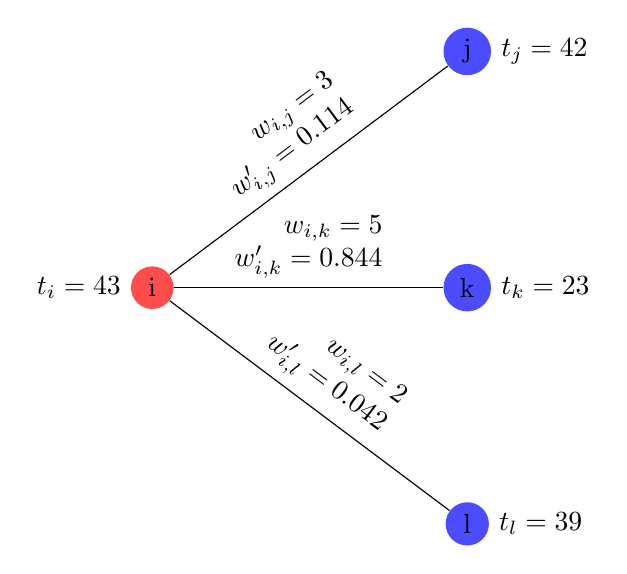
\begin{tikzpicture}[node/.style={circle,fill=red!70,minimum size=1em,inner sep=3pt]}, neighbor/.style={circle,fill=blue!70,minimum size=1em,inner sep=3pt]}]
      \node[node, label=left:{$t_{i} = 43$}] (1) at (-1, -1) {i};
      \node[neighbor, label=right:{$t_{j} = 42$}] (2) at (3, 2.0) {j};
      \node[neighbor, label=right:{$t_{k} = 23$}] (3) at (3, -1) {k};
      \node[neighbor, label=right:{$t_{l} = 39$}] (4) at (3, -4.0) {l};

      \draw (1) -- (2) node [midway, above, sloped, align=right] (a) {$w_{i,j} = 3$ \\ $w'_{i,j} = 0.114$};
      \draw (1) -- (3) node [midway, above, sloped, align=right] (b) {$w_{i,k} = 5$ \\ $w'_{i,k} = 0.844$};
      \draw (1) -- (4) node [midway, above, sloped, align=right] (c) {$w_{i,l} = 2$ \\ $w'_{i,l} = 0.042$};
    \end{tikzpicture}

    \caption[Extended egocentric network example]{Extended egocentric network of the node \(v_{i} \) (red node) and its neighbors \( v_{j} \), \( v_{k} \), and \( v_{l} \) (blue nodes). Each node stores additionally the point in time on which it was last active. For instance, node \(v_{j} \) was last active at \( t = 42 \). Furthermore, the scaled and normalized weights \( w'_{i,j} \) are part of the network. For example, the scaled weight for the tie between \( v_{i} \) and \( v_{j} \) can be calculated by \( w'_{i,j} = \sfrac{\exp(3)}{\exp(3) + \exp(5) + \exp(3)} = 0.114 \). For the sake of simplicity is \( \beta = 1 \) in this example.}
\label{fig:extended-egocentric-network}
\end{figure}


The usage of the softmax function in our model allows for different influence scenarios.
For example, a value of \( \beta = 0 \) (this would correspond to a very high temperature) would scale every weight to the same value, which means that every active neighbor influences a node equally, regardless of the tie strength.
However, it also possible to make \( \beta \) time-dependent (i.e., \( \beta(t) \)), similar to a physical system that is cooling off or heating up.
For instance, for most of our experiments is the temperature at time \( t \) set to the average weight in the integrated network \( G_{T} = \sum_{i=0}^{t} G_{i}\) (i.e., \( \beta(t) = {(\frac{1}{m} \sum_{(i,j) \in E(G_{T})} w_{i,j})}^{-1} \)).
The normalized weights \( w'_{i,j} \) are also part of the extended egocentric network (c.f. \cref{fig:extended-egocentric-network}) and must be updated at the end of every iteration.
The weighted fraction of active neighbors \( \alpha_{i}(t) \) of node \(v_{i} \) at time \( t - 1 \) is then given by

\begin{equation}
    \alpha_{i}(t) = \frac{\sum_{j \in N(v_{i})} \mathbf{1}_{\{t_{j} = t-1\}} \exp(\beta(t) w_{i, j})}{\sum_{j \in N(v_{i})} \exp(\beta(t) w_{i, j})} = \frac{\sum_{j \in N(v_{i})} \mathbf{1}_{\{t_{j} = t-1\}} w'_{i, j}}{\sum_{j \in N(v_{i})} w'_{i, j}},
\end{equation}

where \( \mathbf{1}_{\{x\}} \) is the indicator function, which yields the value \( 1 \) every time the predicate \( x \) is true, otherwise it is \( 0 \).

Next, the weighted fraction of prior active neighbors must be mapped to a peer influence probability in the range \( [0, q] \) using a monotonically increasing function.
One possibility would be the usage of a linear function \( g(\alpha) = q \alpha \) defined for values \(0 \leq \alpha \leq 1 \).
However, this function seems to not capture the peer influence mechanism very well.
On one hand, an additional active neighbor should not be heavily influential when there is already a large portion of neighbors active.
The peer influence should saturate after some fraction of active neighbors is reached.
On the other hand, the peer influence for a node should become noticeable after some threshold of active neighbors is reached.

These requirements can be satisfied by using a sigmoid function.
Similar to~\cite{Walk2016}, the following algebraic sigmoid function \( g \) is used to determine the peer influence for the node \( v_{i} \)

\begin{equation}
    p_{i}(t) = g(\alpha_{i}(t)) = \frac{\alpha_{i}(t) q}{\sqrt{\alpha_{i}^{2}(t) + \theta^2}},
\end{equation}

where the parameter \( q \) is the maximum peer influence, as discussed prior, and \( \theta > 0 \) denotes a critical threshold, which determines the required (weighted) fraction of active neighbors to set the peer influence probability close to its maximum.
Therefore, active neighbors always affect the peer influence probability, but only after a certain point in a significant way.
The satisfaction of the prior described requirements for the function can be verified by examine its first derivative

\begin{equation}
    \frac{\mathrm{d} g}{\mathrm{d} \alpha} = \frac{q \theta^{2}}{{(\theta^2 + \alpha^2)}^{\sfrac{3}{2}}},
\end{equation}

which approaches zero very fast for values grater than \( q \).

Sigmoid functions are usually defined for all real values, since they are often used to re-scale values to the range \([-1, 1] \) or \( [0, 1] \).
However, in our model only input values on the unit interval are relevant and, therefore, the two parameter \( q \) and \( \theta \) should be selected carefully to archive the desired peer influence behavior.
For instance, too large values for \( \theta \) may obstruct the peer influence mechanism critically, since the maximum influence may never be reached, even if \( \alpha = 1 \).
\Cref{fig:peer-influence-sigmoid} shows the discussed sigmoid function with different values for the critical threshold.


\myfig{peer-influence-sigmoid}
      {width=0.75\textwidth}
      {Depiction of the sigmoid function that is used to calculate the peer influence probability \(p_{i} \) of a node based on its (weighted) fraction of active neighbors \( \alpha \) for different values of the critical threshold \( \theta \). The maximum possible peer influence probability in this example is fixed to \( q = 0.10 \). The critical threshold determines how fast the maximum peer probability can be reached. Values in the range between 5\% and 20\% seem to be a sound choice, since already a small number of influential neighbors should suffice to have an notable effect on a user.}
      {Peer influence sigmoid function examples}
      {fig:peer-influence-sigmoid}


The self-activation mechanism for nodes must be adapted as well.
The simple biased coin flip becomes a more sophisticated two-step random experiment.
First, like in the base model, a biased coin is tossed to determine if a node becomes active with probability that corresponds to its activity potential.
If this first random experiment fails, the node gets a second chance to become active by himself.
This is done by calculating the nodes' peer influence probability and tossing another biased coin.
Therefore, the total probability for a node \( v_{i} \) to become active at time \( t \) can be expressed by

\begin{equation}
    \prob{v_i \text{ becomes active}} = a_{i} + (1 - a_{i}) p_{i}.
\end{equation}

This concludes the definition of the extension for the community-oriented activity-driven time-varying network model that introduces a new peer influence mechanism.
\Cref{tbl:all-model-parameter} contains an overview of all model parameter and their origin.
Note that many of them (e.g., \( \Delta t \), \( \eta \), \ldots) have reasonable default values assigned to them in the context of our work.


\begin{table}
\centering
\begin{tabular}{lp{10cm}}
\toprule
\textbf{parameter} & \textbf{description} \\
\midrule
\multicolumn{2}{c}{activity-driven framework} \\
\midrule
\( n \) & The number of nodes in the network. \\
\( f(x) \) & The probability distribution for the activity potentials of the nodes. It yields a positive probability for values in the range of \( [\varepsilon, 1] \). \\
\( \varepsilon \) &  The lower bound of the activity potential. It should be \( 0 < \varepsilon \ll 1 \). \\
\( \Delta t \) &  The length of the time window in each iteration. \\
\( \eta \) &  A rescaling factor for the activity potential to adjust the average number of active nodes in each iteration. \\
\( m \) & The number of contacts a node initiates, once it become active. \\
\midrule
\multicolumn{2}{c}{community structure extension} \\
\midrule
\( p_{\Delta} \) & The probability to form a triangle when establishing a new tie. \\
\( p_{d} \) & The probability for node to get deleted in a iteration. \\
\( \delta \) & The constant value that is added to the tie strength when it is reinforced. \\
\( c \) &  The memory constant, which influences the probability to form a new tie.\\
\midrule
\multicolumn{2}{c}{peer influence extension} \\
\midrule
\( \beta \) & Inverse temperature parameter for the softmax rescaling of the weights. This parameter may also be time dependent. \\
\( q \) & The maximum possible peer influence probability that a node can receive. \\
\( \theta \) & The critical threshold for the peer influence. \\
\bottomrule
\end{tabular}

\caption[Overview proposed model parameter]{An overview of the parameter set of the proposed model.}
\label{tbl:all-model-parameter}
\end{table}
